%
% introduction.tex
%
% Copyright (C) 2022 by Universidade Federal de Santa Catarina.
%
% GNSS Networks Based on Small Satellites
%
% This work is licensed under the Creative Commons Attribution-ShareAlike 4.0
% International License. To view a copy of this license,
% visit http://creativecommons.org/licenses/by-sa/4.0/.
%

%
% \brief Introduction section.
%
% \author Gabriel Mariano Marcelino <gabriel.mm8@gmail.com>
%
% \version 0.0.0
%
% \date 2019/11/30
%

\section{Introduction} \label{sec:introduction}

Este trabalho tem como proposta o estudo, verificação de viabilidade e implementação de uma rede de um Sistema Global de Navegação por Satélite (\textit{Global Navigation Satellite System}, GNSS) baseada em satélites de pequeno porte, considerando especialmente os nanossatélites, ou em específico os CubeSats.

\cite{nanosatseu}

\begin{figure}[!ht]
    \begin{center}
        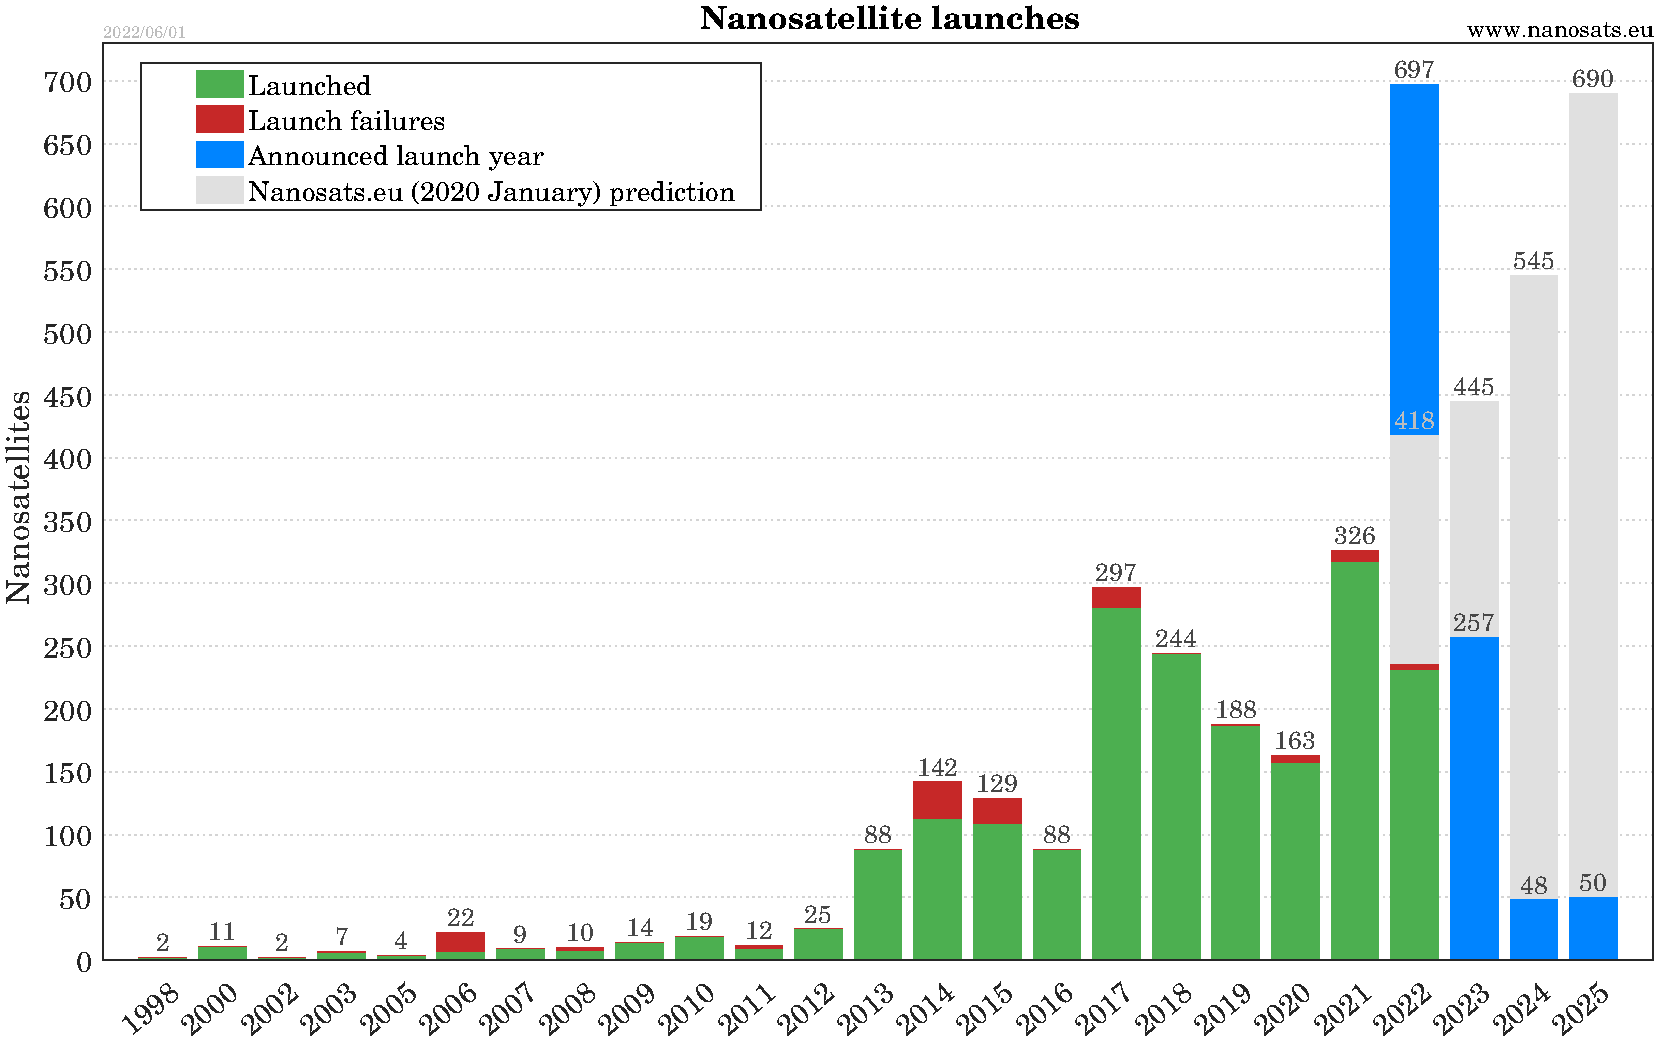
\includegraphics[width=\columnwidth]{figures/Nanosats_years_2022-06-01}
        \caption{Nanosatellite launches (2022/06/01).}
        \label{fig:cubesat-launches}
    \end{center}
\end{figure}

\begin{figure}[!ht]
    \begin{center}
        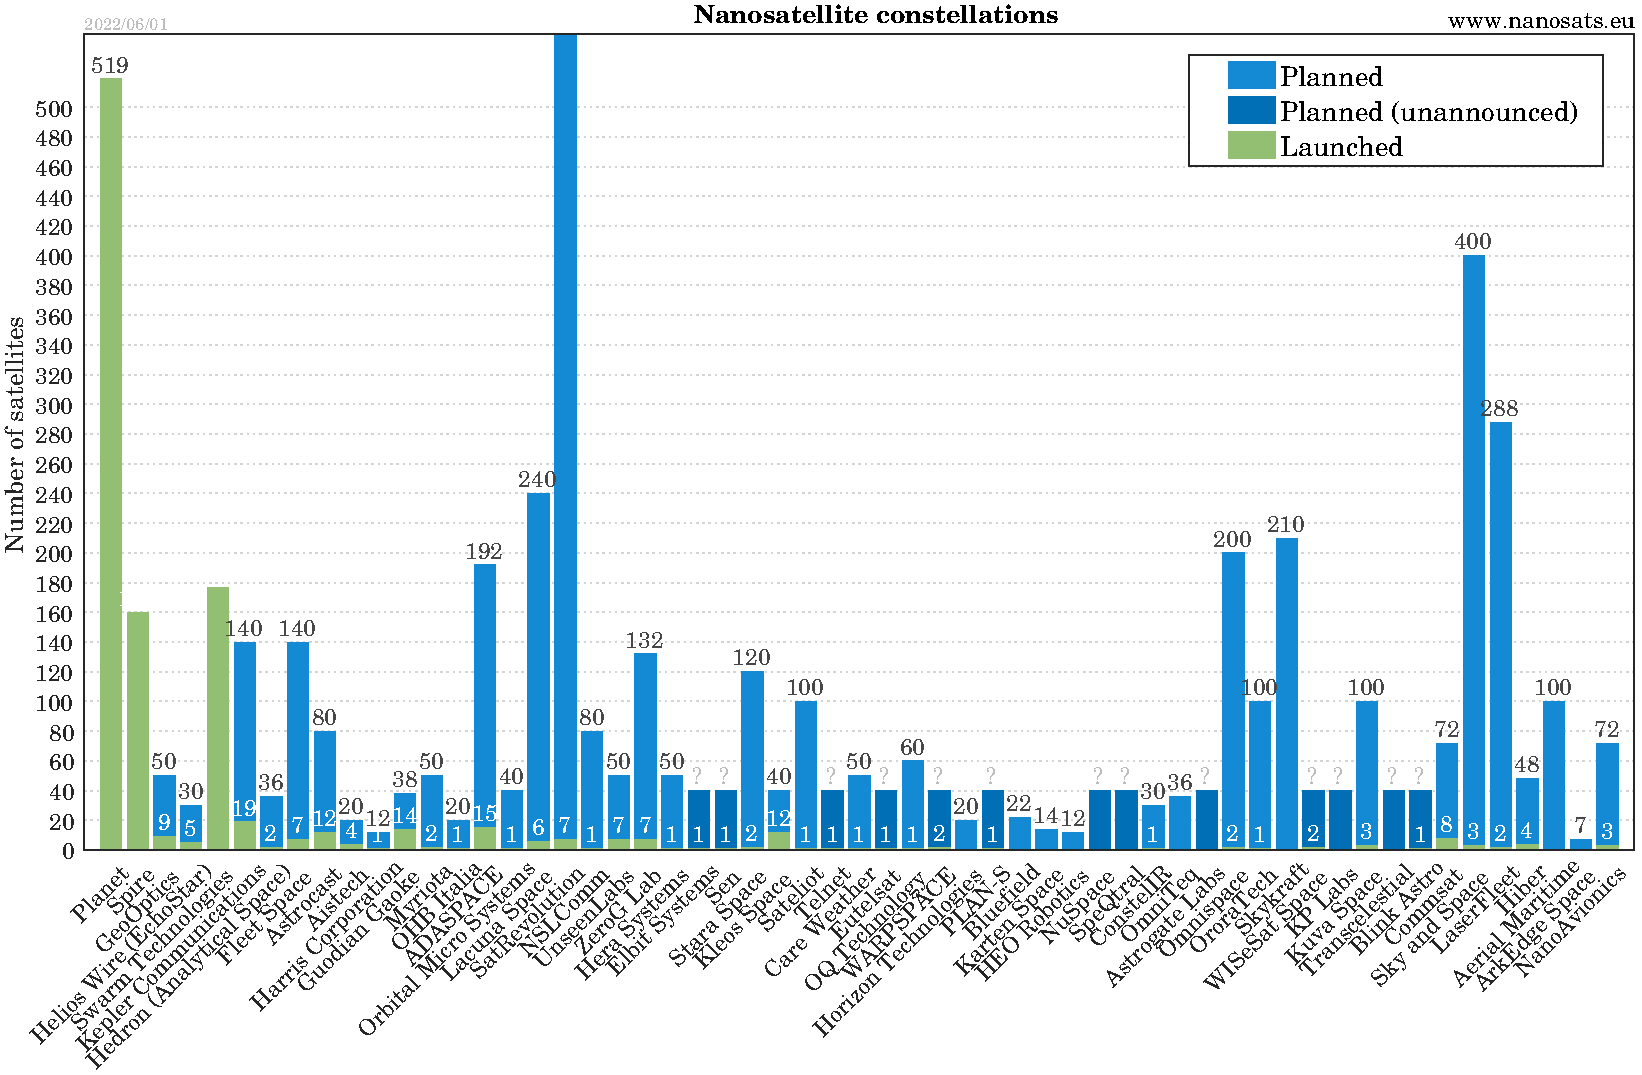
\includegraphics[width=\columnwidth]{figures/Nanosats_constellations_2022-06-01}
        \caption{Nanosatellite constellations (2022/06/01).}
        \label{fig:constellations}
    \end{center}
\end{figure}
